\documentclass{standalone}
\pagestyle{empty}
\usepackage{tikz}
\usetikzlibrary{arrows.meta,bending}

\begin{document}
\noindent
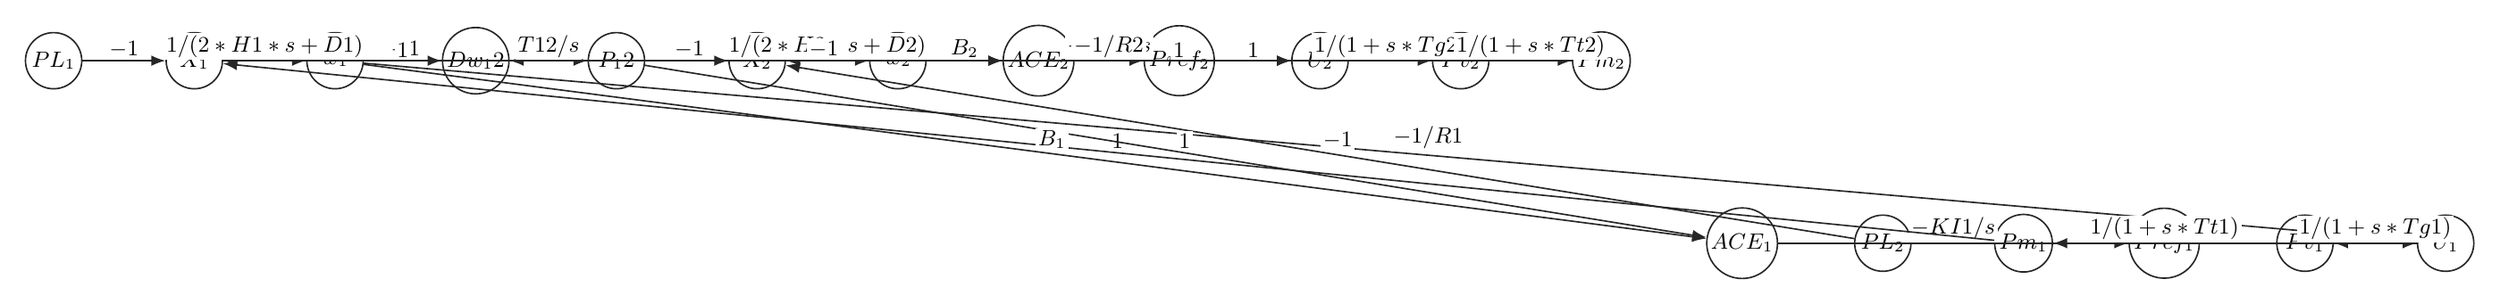
\begin{tikzpicture}[
  >=Latex,
  ->,
  semithick,
  every node/.style={font=\small},
  signal node/.style={circle,draw,minimum size=8mm,inner sep=1pt,fill=white},
  io node/.style={rectangle,rounded corners=2pt,draw,minimum width=8mm,minimum height=6mm,inner sep=2pt,fill=gray!8},
  every path/.style={draw=black!85},
  edge label/.style={fill=white,inner sep=1pt,text=black},
]
\node[signal node] (PL1) at (0.0,0.0) {$PL_1$};
\node[signal node] (X1) at (2.0,0.0) {$X_1$};
\node[signal node] (w1) at (4.0,0.0) {$w_1$};
\node[signal node] (Dw12) at (6.0,0.0) {$Dw_12$};
\node[signal node] (P12) at (8.0,0.0) {$P_12$};
\node[signal node] (X2) at (10.0,0.0) {$X_2$};
\node[signal node] (w2) at (12.0,0.0) {$w_2$};
\node[signal node] (ACE2) at (14.0,0.0) {$ACE_2$};
\node[signal node] (Pref2) at (16.0,0.0) {$Pref_2$};
\node[signal node] (U2) at (18.0,0.0) {$U_2$};
\node[signal node] (Pv2) at (20.0,0.0) {$Pv_2$};
\node[signal node] (Pm2) at (22.0,0.0) {$Pm_2$};
\node[signal node] (ACE1) at (24.0,-2.6) {$ACE_1$};
\node[signal node] (PL2) at (26.0,-2.6) {$PL_2$};
\node[signal node] (Pm1) at (28.0,-2.6) {$Pm_1$};
\node[signal node] (Pref1) at (30.0,-2.6) {$Pref_1$};
\node[signal node] (Pv1) at (32.0,-2.6) {$Pv_1$};
\node[signal node] (U1) at (34.0,-2.6) {$U_1$};
\draw (ACE1) -- node[edge label,midway,above] {$-KI1/s$} (Pref1);
\draw (Pref1) -- node[edge label,midway,above] {$1$} (U1);
\draw (w1) -- node[edge label,midway,above right] {$-1/R1$} (U1);
\draw (U1) -- node[edge label,midway,above] {$1/(1+s*Tg1)$} (Pv1);
\draw (Pv1) -- node[edge label,midway,above] {$1/(1+s*Tt1)$} (Pm1);
\draw (Pm1) -- node[edge label,midway,above right] {$1$} (X1);
\draw (PL1) -- node[edge label,midway,above] {$-1$} (X1);
\draw (P12) -- node[edge label,midway,above] {$-1$} (X1);
\draw (X1) -- node[edge label,midway,above] {$1/(2*H1*s + D1)$} (w1);
\draw (ACE2) -- node[edge label,midway,above] {$-KI2/s$} (Pref2);
\draw (Pref2) -- node[edge label,midway,above] {$1$} (U2);
\draw (w2) -- node[edge label,midway,above] {$-1/R2$} (U2);
\draw (U2) -- node[edge label,midway,above] {$1/(1+s*Tg2)$} (Pv2);
\draw (Pv2) -- node[edge label,midway,above] {$1/(1+s*Tt2)$} (Pm2);
\draw (Pm2) -- node[edge label,midway,above] {$1$} (X2);
\draw (PL2) -- node[edge label,midway,above right] {$-1$} (X2);
\draw (P12) -- node[edge label,midway,above] {$1$} (X2);
\draw (X2) -- node[edge label,midway,above] {$1/(2*H2*s + D2)$} (w2);
\draw (w1) -- node[edge label,midway,above] {$1$} (Dw12);
\draw (w2) -- node[edge label,midway,above] {$-1$} (Dw12);
\draw (Dw12) -- node[edge label,midway,above] {$T12/s$} (P12);
\draw (P12) -- node[edge label,midway,above right] {$1$} (ACE1);
\draw (w1) -- node[edge label,midway,above right] {$B_1$} (ACE1);
\draw (P12) -- node[edge label,midway,above] {$-1$} (ACE2);
\draw (w2) -- node[edge label,midway,above] {$B_2$} (ACE2);
\end{tikzpicture}
\end{document}
